\chapter{Introduction}
\lhead{\emph{Introduction}}

The desire for a feeling of presence \cite{presence} within a space that is not your own is one that drives much technological innovation. Whether it be within a virtual space such as in video games or immersion therapy, or within a different real world location as in telerobotics, greater presence allows the user to more naturally and intuitively interact with the presented environment as if they were truly there. In telerobotics in particular, where the aim can often be to interact with very dangerous or industrial environments, intuitive control is essential to safe and effective operation.

Virtual Reality (VR) is a technology spearheaded by the video games industry for use in immersive gaming application. Through the use of a tracked headset, giving the user the ability to freely look around a 3D space, it provide unparalleled presence within a virtual world- comparable to presence within a real, physical space \cite{loomis2016presence,McGlynn}. To be able to incorporate VR into teleoperation is therefore desirable, however, sending a video feed to the headset as if it were a normal monitor has been found to lead to motion sickness \cite{han2017design}. This is due to VR's high frame rate and low latency requirements. It's widely accepted that for a VR application to not cause motion sickness and headaches due to frame rate, it must maintain at least 90 frames per second (fps) \cite{FrameRate}; a minimum of 60 fps can also be acceptable \cite{Borg2013UsingAG}, but generally only for applications with little motion or when used by people with lower susceptibility to motion sickness. Unfortunately, to transmit 90 fps from a stereo camera rig (two images are required to perceive 3D) to the computer running the VR application has bandwidth requirements too high to be currently implementable outside the most expensive of designs.

The ability to look around the space independently is a major factor in providing presence to the user in VR. This can be achieved by mounting the stereo camera rig on a gimbal, however to build a gimbal that is able to track the angle of the user's head accurately and with low latency is, once again, expensive and challenging \cite{DORA}; if not implemented perfectly the user would experience significant sickness and dissociation from the space.

The aim of this project is to design and implement a VR based teleoperation system that utilises data abstraction to minimise the outlined technical issues, providing the foundations for future systems to be able to provide true presence to the user. To achieve this, each image is reduced down to its most essential features, reducing its size and therefore the required bandwidth significantly. Each image pair must then transmitted to a server and combined into a single 3D model of the space that could be looked around freely through the VR headset. As the camera feed is converted to a 3D model rather than displayed directly as images, the headset could run at the full 90fps even if the model is updating at a much slower rate.

The system (outlined in Figure \ref{fig:outline}) consists of 2 platforms- a server that runs a VR environment and reads user input, and a rover platform that is controlled from said environment and supplies the abstracted images the environment is built from. The rover (Figure \ref{fig:marvin}) is a simple drivable platform with a stereo camera gimbal mounted on it (adapted from one produced by previous students \cite{gimble}), and is the subject of Chapter \ref{chapter:rover}. The server is a powerful PC running Windows 10 \cite{windows} and a HTC Vive. The design of the program the server runs is the subject of Chapter \ref{chapter:server}. The data abstraction algorithm the system uses is novel, so its design and development is initially discussed in isolation in Chapter \ref{chapter:abstract} and then its application within the system addressed in Chapter \ref{chapter:rover}. The full system will be evaluated in Chapter \ref{chapter:eval}.

\begin{figure}[H]
    \begin{center}
      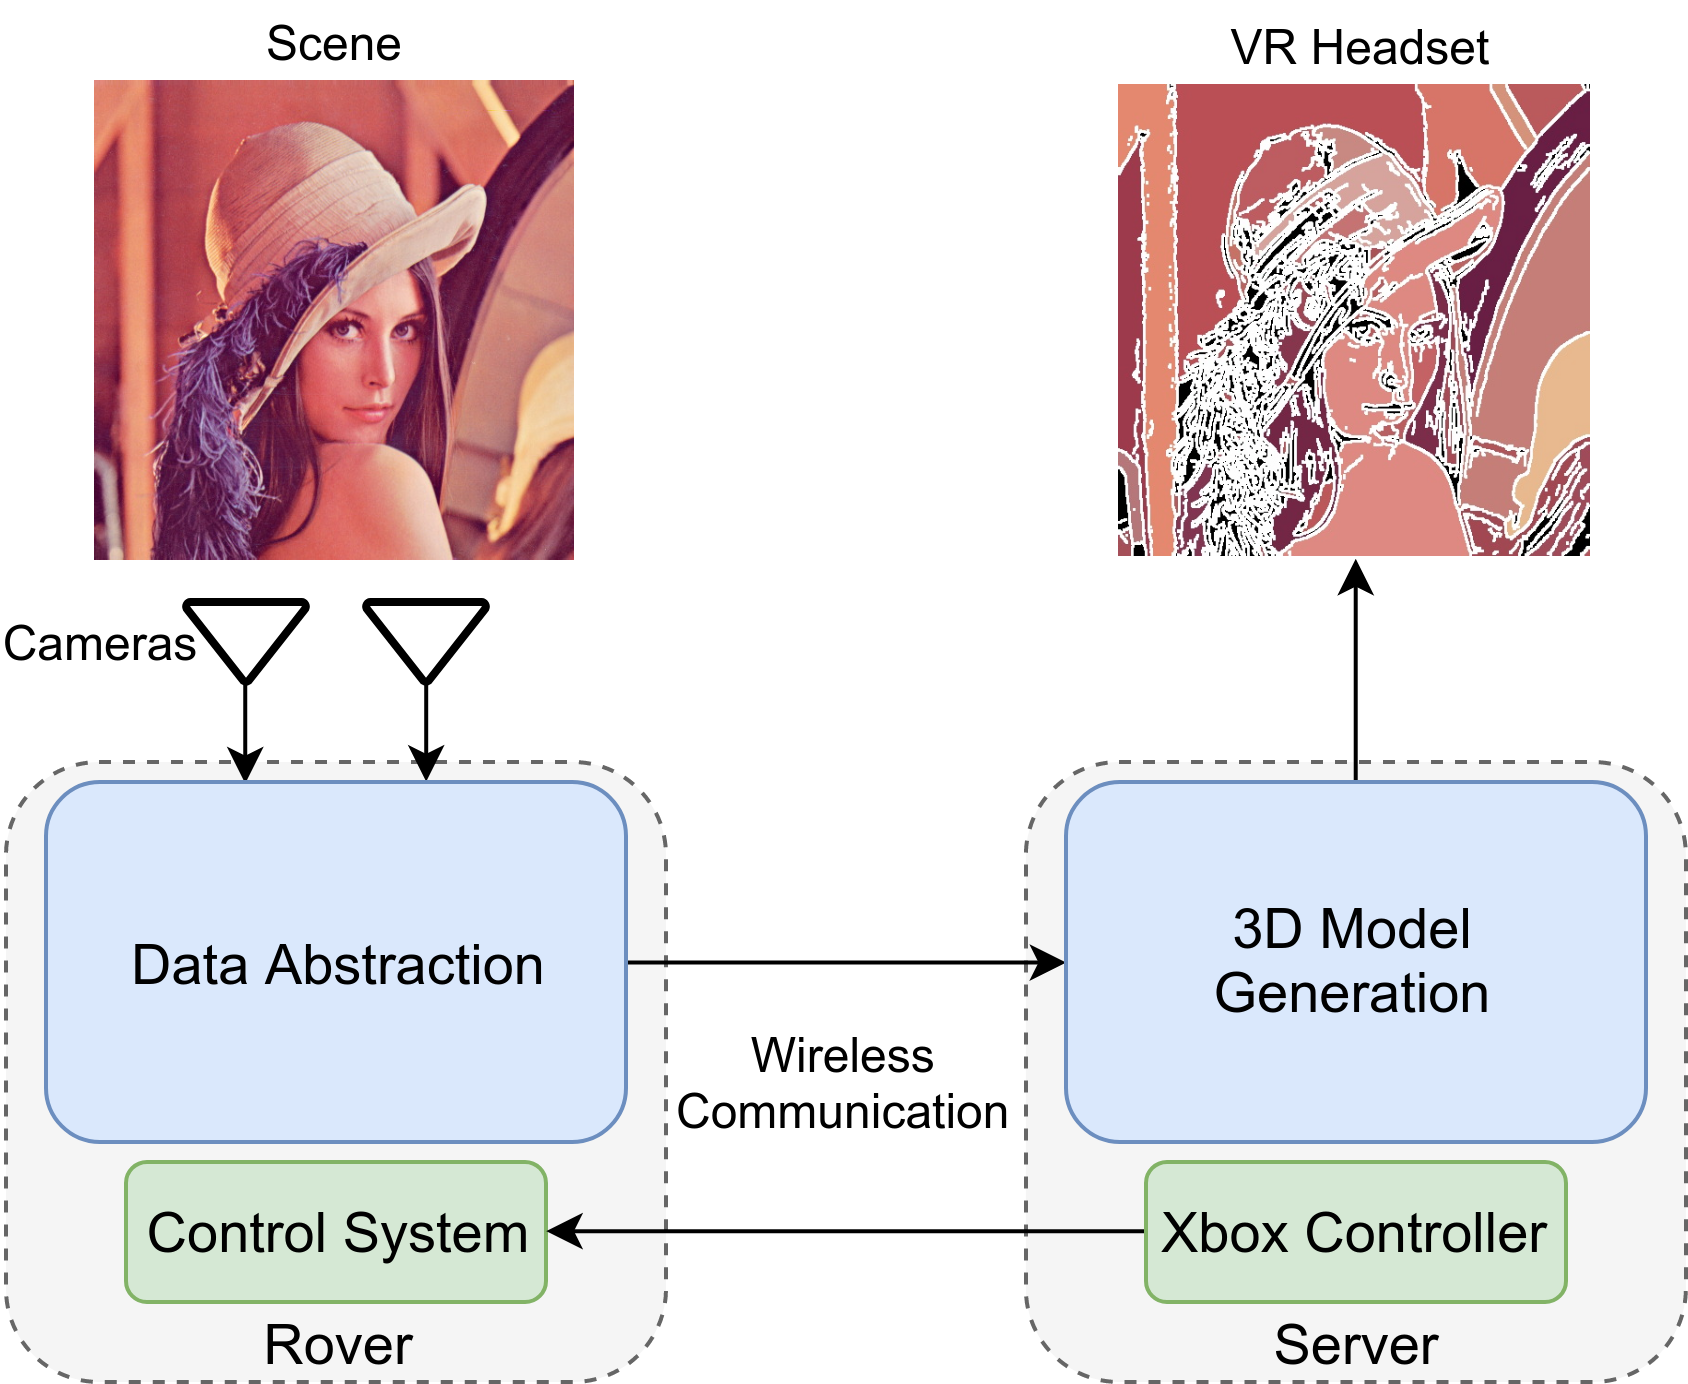
\includegraphics[width=0.9\textwidth]{Figures/Outline.png}
      \caption[System Outline]{System Outline.\textcolor{red}{[REPLACE PICS]}}
      \label{fig:outline}
    \end{center}
\end{figure}

\begin{figure}[H]
    \begin{center}
      \includegraphics[width=0.6\textwidth]{Figures/marvin.jpg}
      \caption[Rover Picture]{Rover Picture.\textcolor{red}{[NEEDS MANY UNAMBIGUOUS PICS]}}
      \label{fig:marvin}
    \end{center}
\end{figure}